\section{Why Coarsening a Filter is Bad}
\label{sec:coarsen}

% \begin{figure}[t]
% {\eightpoint
% \begin{verbatim}
% float->float stateful filter WeightCalc(int n)
% {
%   float[n] window;
%   int windowPos;

%   ...

%   // the input stream is multiplied with the weights
%   work push 2 pop 2
%   {

%     push(pop() * window[windowPos]);
%     push(pop() * window[windowPos]);

%     windowPos++;
%     if(windowPos >= n)
%     {
%       windowPos = 0;
%     }
%   }
% }
% \end{verbatim}
% \caption{MPD filter that multiplies stream values with weights.\protect\label{fig:weight-calc}}}
% \end{figure}


\begin{figure*}[t!]
\centering
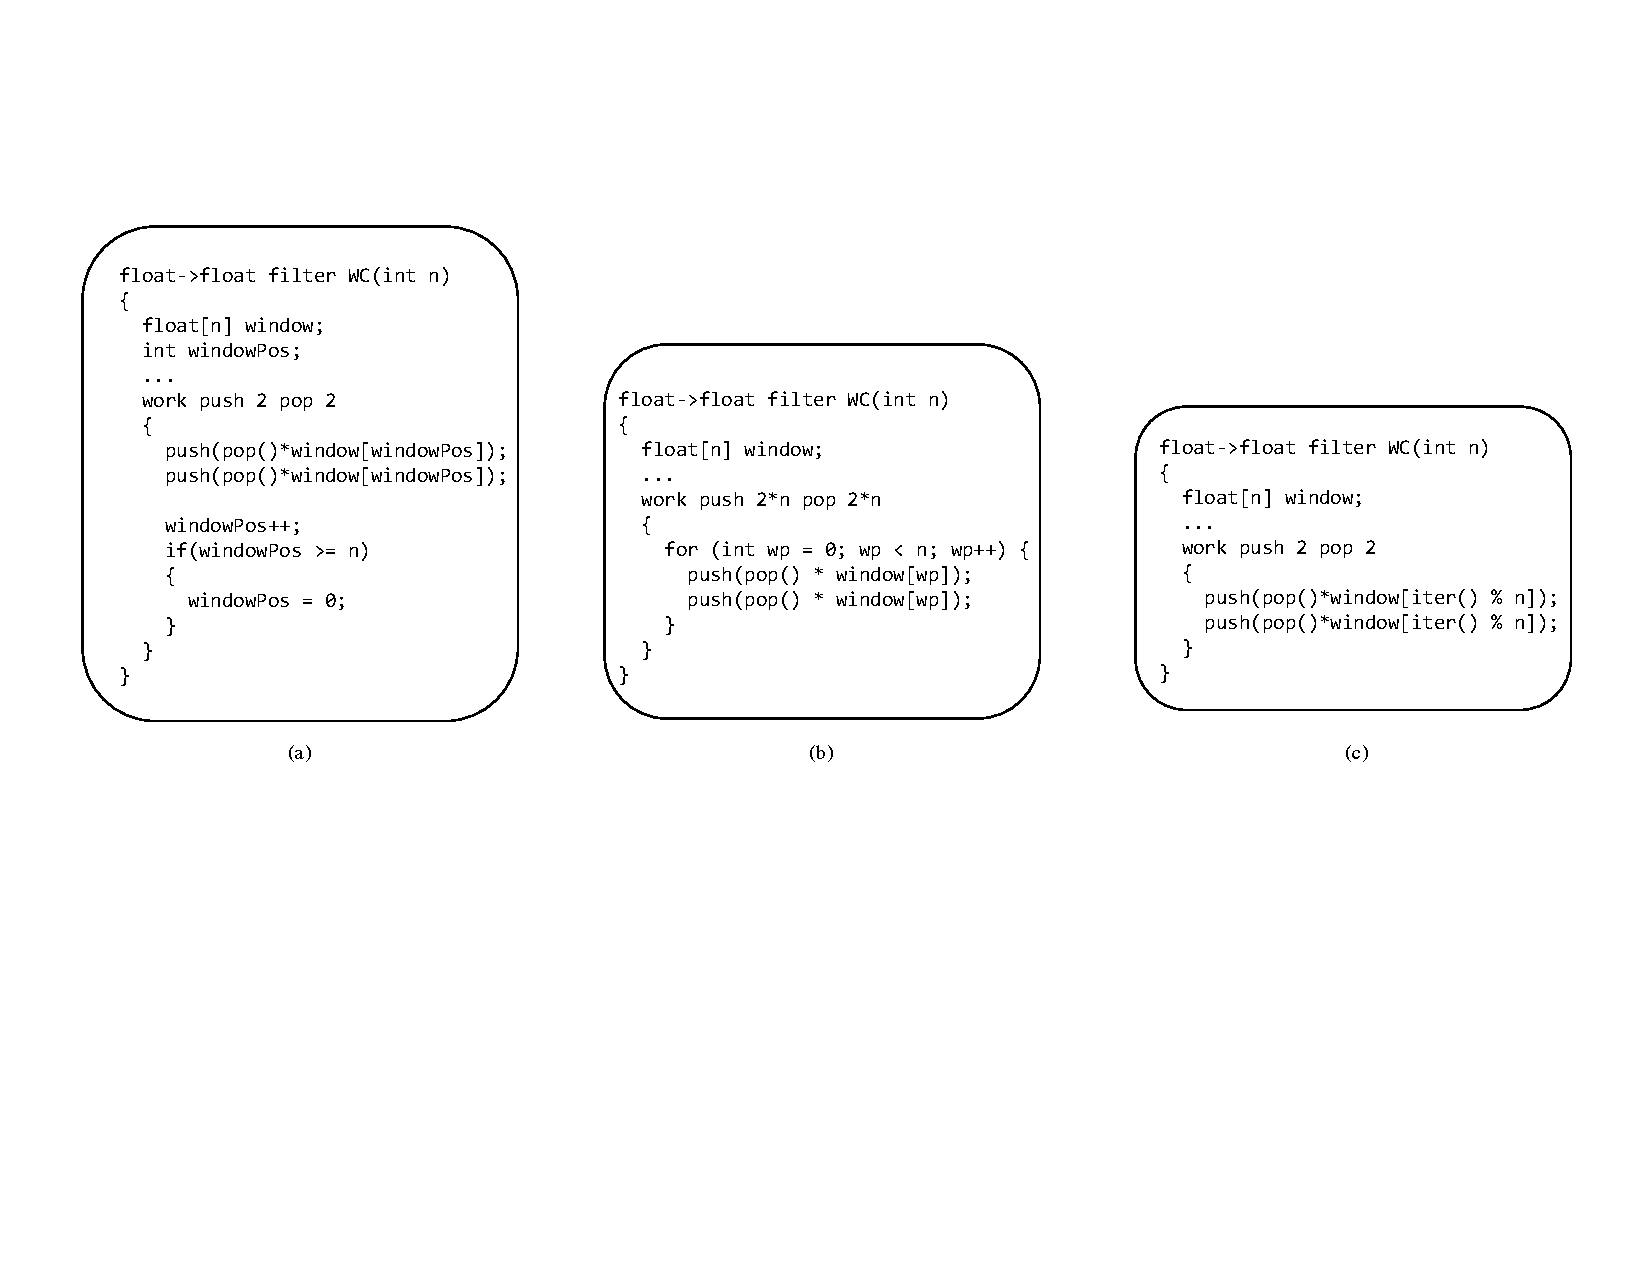
\includegraphics[width=6.5in]{figures/weights-calc-example.pdf}
\caption{Three versions of the weights calculation filter from Medium Pulse Dopler (MPD) (a) is the original filter with explicit induction variable state.  (b) is a coarsened version without state. (c) is a version that utilizes the {\tt iter()} keyword to avoid state.\protect\label{fig:wc-example}}
\end{figure*}


n = 32

One could write the induction filters given above at a more coarse granularity
such that the filter is pushing and popping ???? number of items.
Since the period of the filter is known at compile-time, though
parameterized, the push and pop rate could be equal to the period and
[explain how to coarsen].  This approach, however, is inferior because
of the following:

* The programmer grasped the algorithm and implemented the application
at the fine granularity.  A language should constrain the programmer
as little as possible for the sake of performance.

* The coarse-granularity implementation requires larger input and
output buffers to implement because of the larger push and pop rates.
Larger buffers occupy more of the cache and could evict filter data or
instructions are needed during execution.  Thus there could be more
access to longer latency memory hierarchies.

* Larger input and output rates also interact with the steady-state
scheduling algorithm.  Since the scheduling algorithm is performing
many cascading LCMs, a single filter with large input and output rates
will increase the multiplies of all filters of the application,
requiring more buffering and increasing latency.